
The most stringent limits on sparticles generally come from inclusive
searches for strongly produced squark and gluinos, in particular to
the all hadronic final states. These searches are performed within the
inclusive squark and gluino sub-group, composed of approximately 140
members and split into eight paper streams based on the number of jets
and lepton flavors in the final state.  UTA has been envolved in these
searches since beginning of Run 1, twice convening this subgroup (UTA
postdocs David Cote and Heelan), and most recently supervising several
public papers and conference notes for ICHEP
2016~\cite{Aad:2016jxj,Aaboud:2016zdn,Aad:2016qqk,ATLAS-CONF-2015-082,Aad:2016tuk,Aad:2016eki,Aaboud:2016zpr,ATLASCollaboration:2016wlb,ATLAS-CONF-2016-078,ATLAS-CONF-2016-054,ATLAS-CONF-2016-037,ATLAS-CONF-2016-052,ATLAS-CONF-2016-066,ATLAS-CONF-2016-095}. Heelan
also directly contributed to the search for SUSY in all hadronic
states.



Between 2010-15, Farbin's ECRP grant supported introduction of novel
``event view'' techniques to search for SUSY, starting with the Razor
reconstruction technique~\cite{Rogan:2010kb} in 2011\cite{Aad:2012naa}
and 2012 ~\cite{Aad:2015iea}. The fourth iteration of this line of
searches, based on an extension called the Recursive Jigsaw
Reconstruction (RJR), was performed in Run 2 for ICHEP
2016~\cite{ATLAS-CONF-2016-078} and was the final topic of Bullock's
now completed PhD thesis~\cite{}. In the RJR views all final state
objects are grouped together in hemispheres made with an underlying
assumption about how the decay is proceeding. An uncorrelated basis of
variables are constructed based on energy scales (masses, transverse
quantities) and scaleless variables (like angles between hemispheres
and ratios of energy scale variables). Looking in all hadronic final
states the RJR method has shown to select only about 50\% of the
events in common with the standard search variables constructed from
detector variables (missing transverse momentum, $H_\mathrm{T}$,
etc.), and hence extend the phase space being searched. [And
  lengthening the statistical reach of such search, if probably
  combined.]


An example of the views used in the latest analysis presented at
ICHEP2016 are shown in Figure~\ref{fig:RJRTrees}.  Using these views
signal regions were designed to search for SUSY produced by squark or
gluino pair production and direct decay to final states containing
jets and the lightest supersymmetric particle.
Figure~\ref{fig:ICHEPLimits} shows that in general across simplified
model planes representing these type of models the new RJR method had
an expected sensitivity similar to that of the standard detector-based
variables.  In this version of the analysis the RJR method included a
view targeting the compressed regions of phase space where all final
state objects are assumed to recoil off an ISR
jet~\cite{Jackson:2016mfb}.  As can also be seen in
Figure~\ref{fig:ICHEPLimits} the RJR did extend the limits with
respect to the effective mass analysis in the compressed region due to
this additional targetted ISR event view.  For the squark-squark
production case (Figure~\ref{fig:ICHEPLimits} (left)) this can be seen
around $m_{\tilde{q}} = 700~\mathrm{GeV}$ for $\Delta m(\tilde{q} -
\chi_1^0) = 100~\mathrm{GeV}$, where the reach was extended by about
50~GeV.  And for gluino pair production (Figure~\ref{fig:ICHEPLimits}
(right)) this extension of the limits of about 50~GeV happened around
$m_{\tilde{g}} = 925~\mathrm{GeV}$ for $m_{\chi_1^0} =
875~\mathrm{GeV}$


\begin{figure}[tb]
\centering
\subfigure{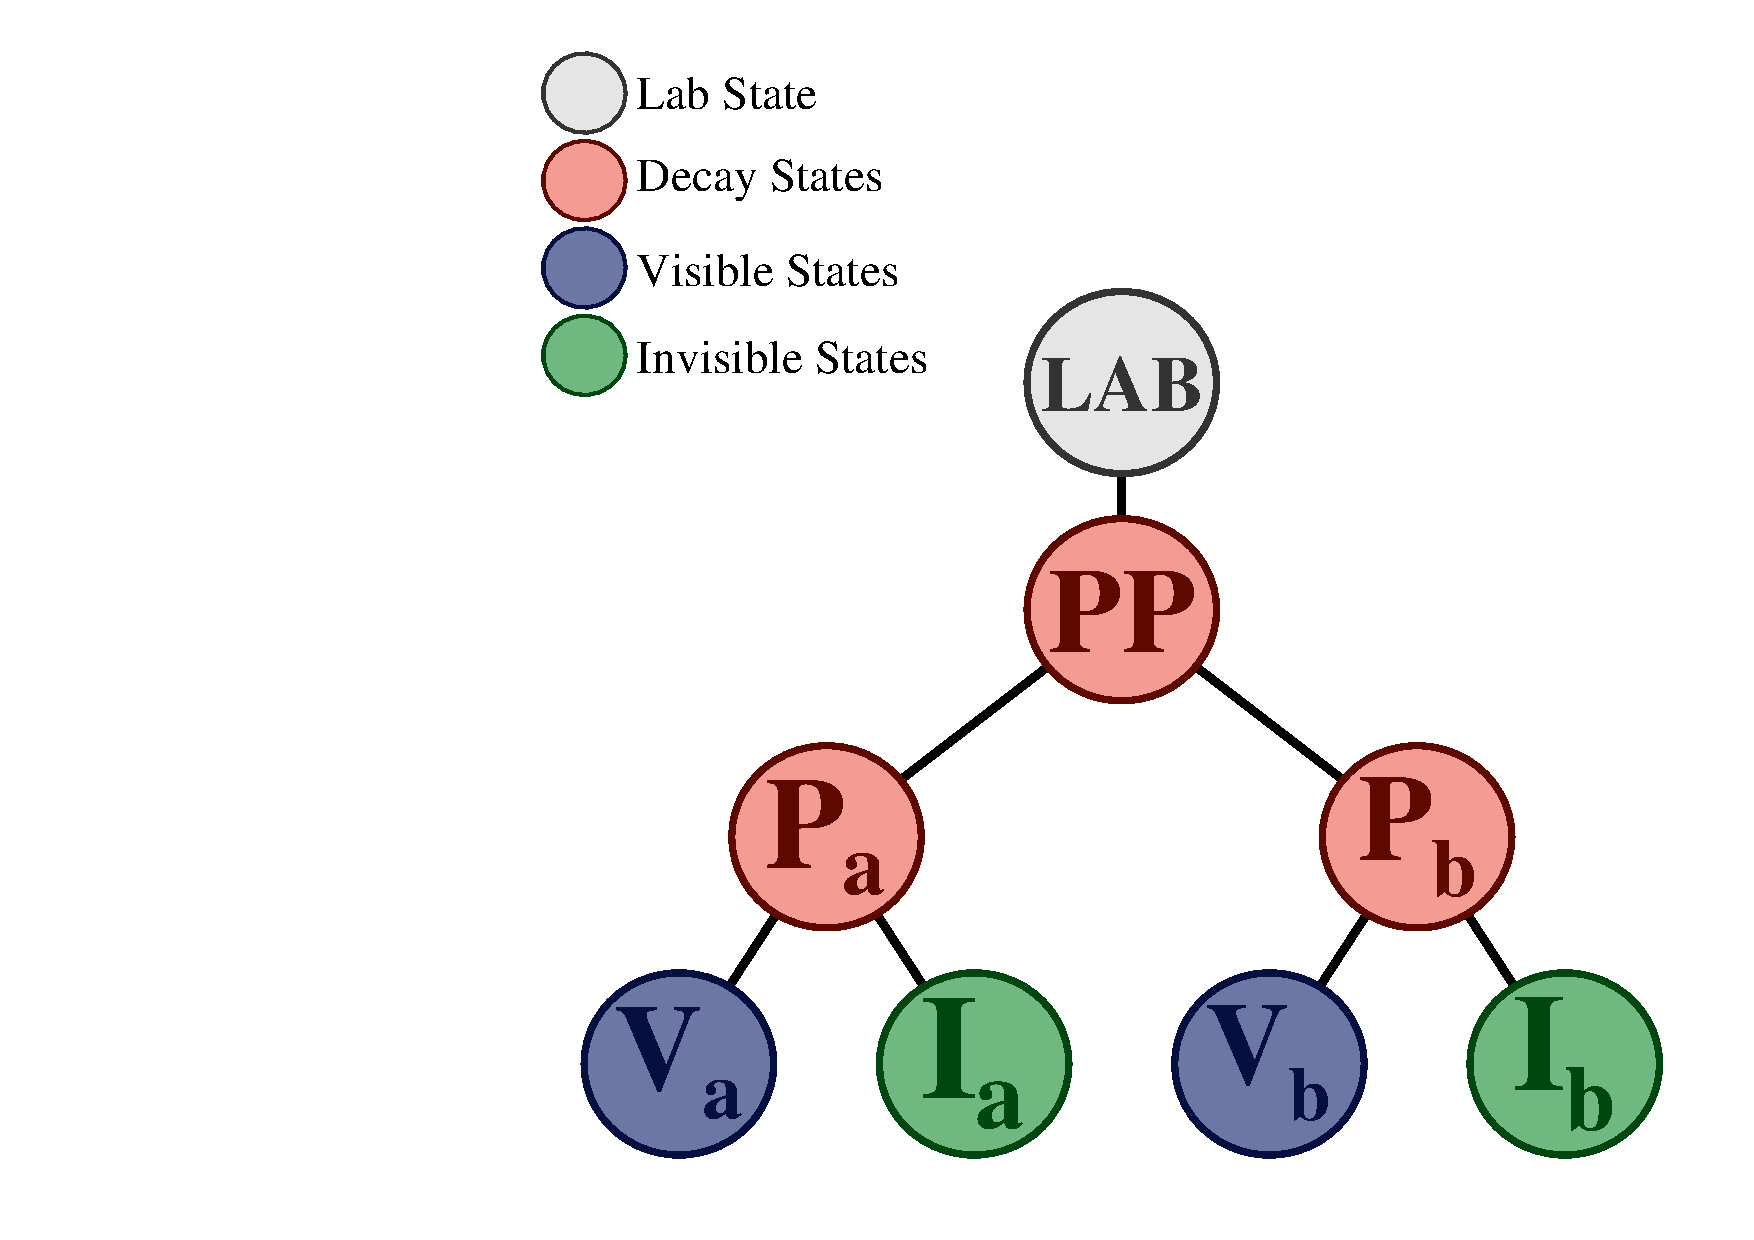
\includegraphics[width=0.30\textwidth]{Figures/RJRtree_DiSparticle.pdf}}
\subfigure{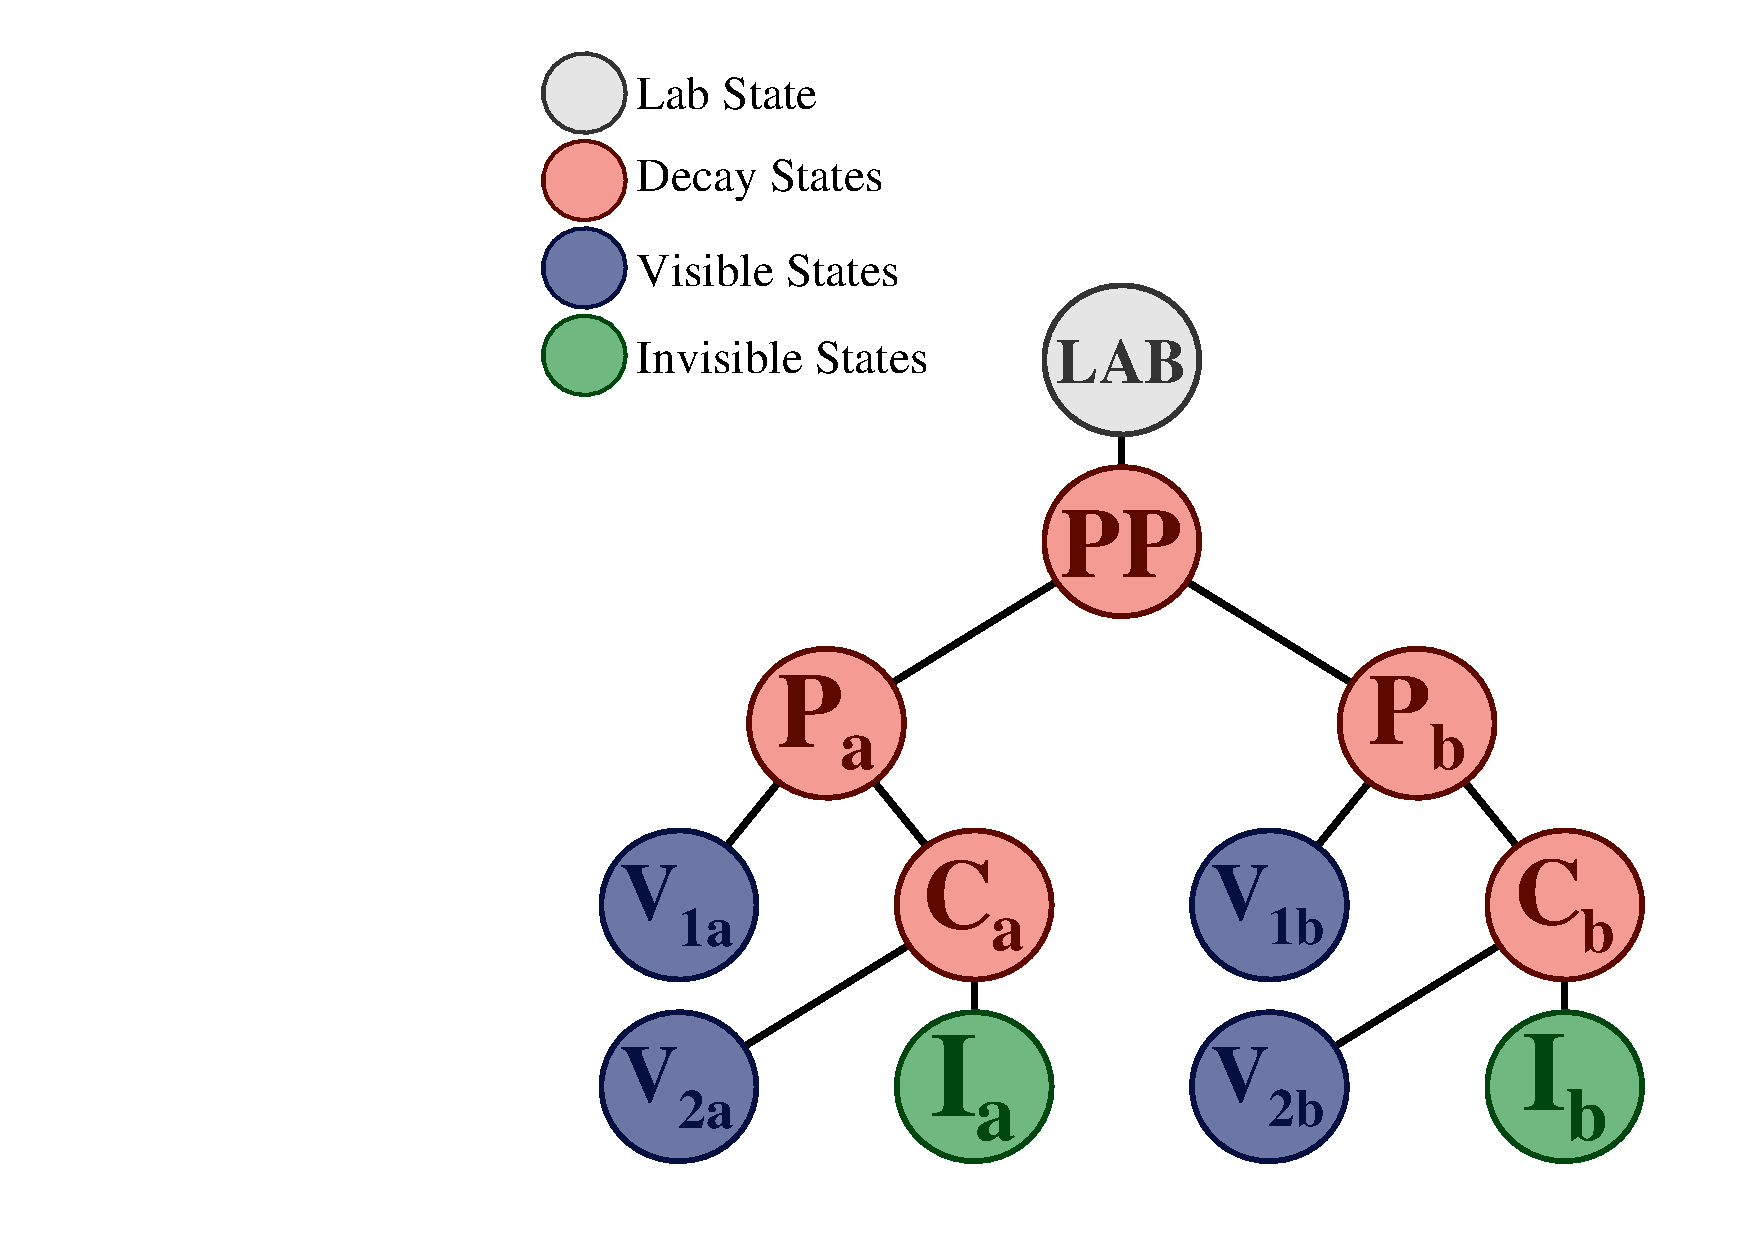
\includegraphics[width=0.30\textwidth]{Figures/RJRtree_DiGluino.pdf}}
\subfigure{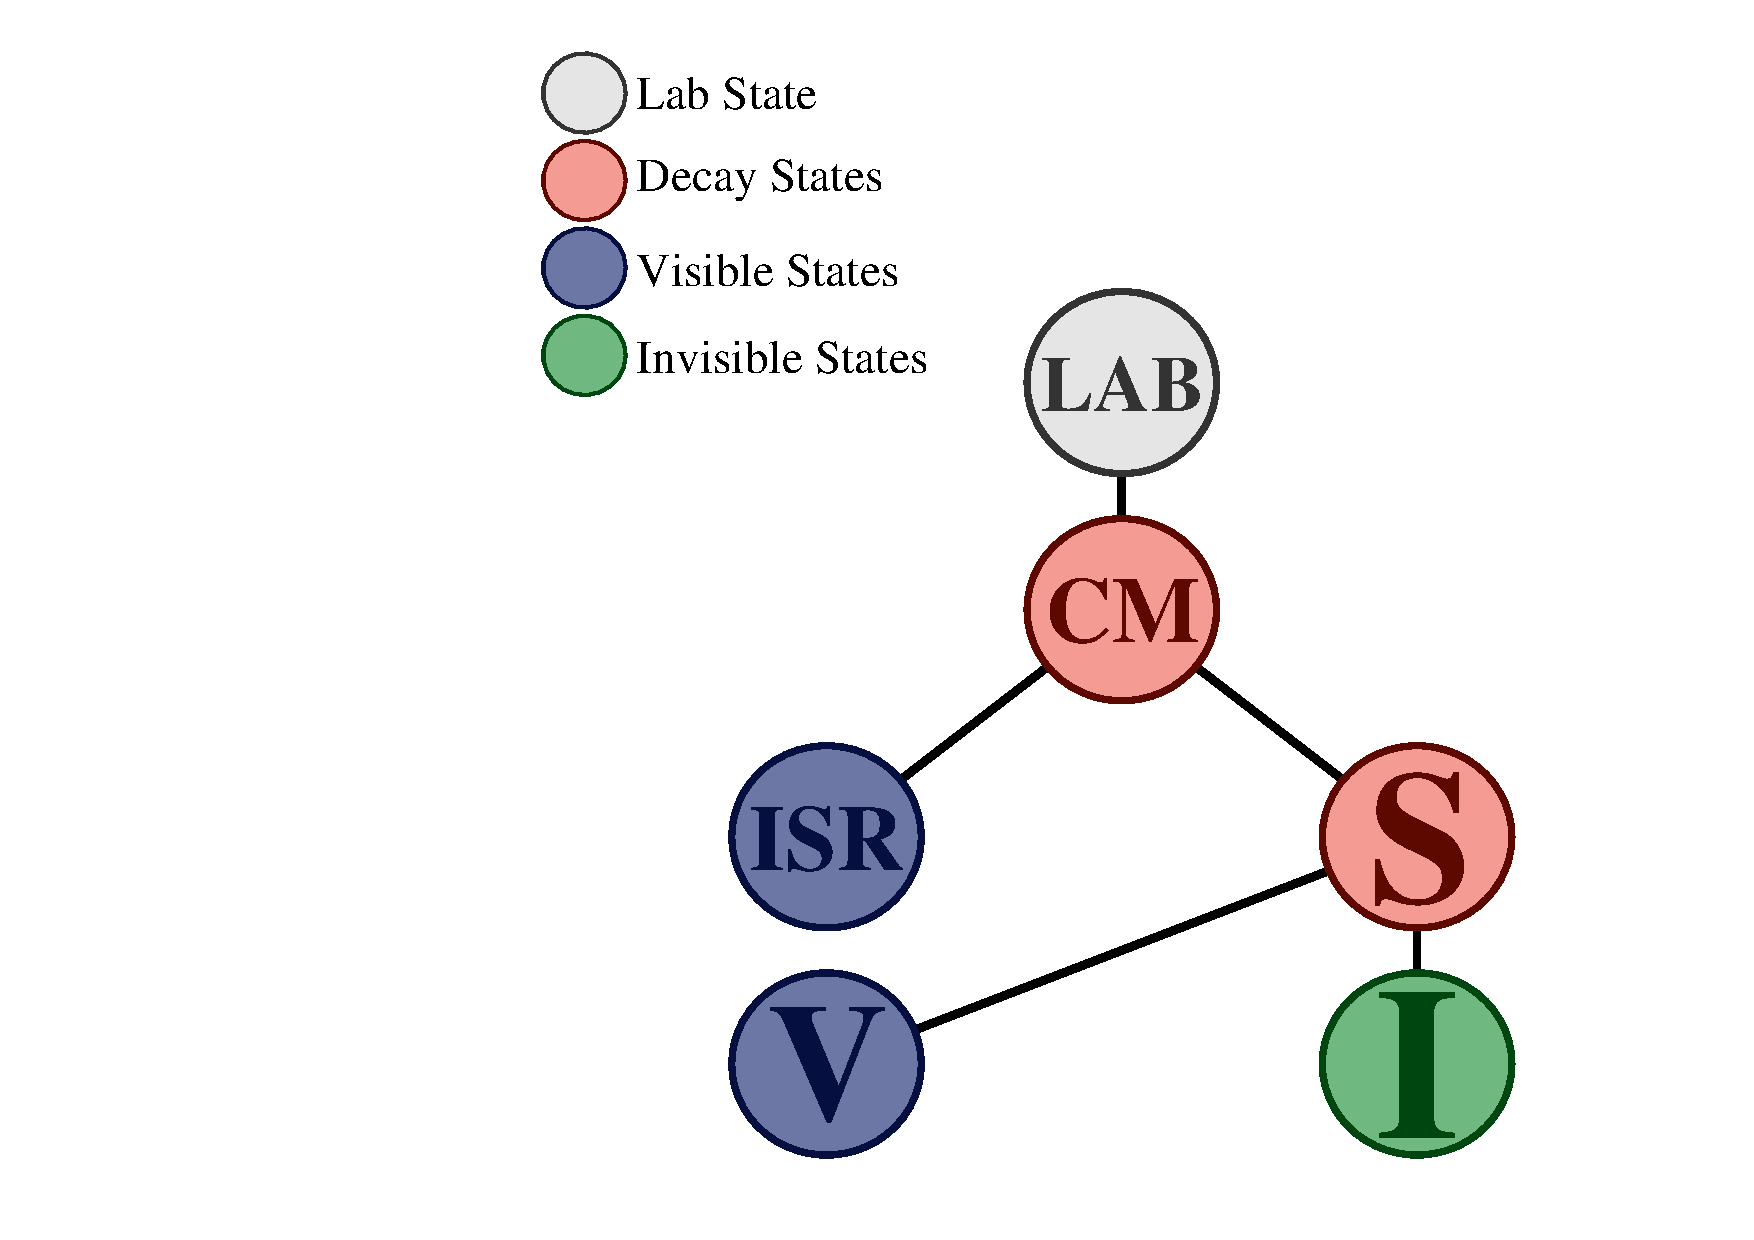
\includegraphics[width=0.30\textwidth]{Figures/RJRtree_Compressed.pdf}}
\caption{\label{fig:RJRTrees} Recursive Jigsaw Reconstruction event views for three scenarios: (a) Two sparticles ($P_{a}$ and $P_{b}$) are pair-produced with each decaying to one or more visible particles ($V_{a}$ and $V_{b}$) which are reconstructed in the detector, and two systems of invisible particles ($I_{a}$ and $I_{b}$) whose four-momenta are only partially constrained. (b) An additional level of decays can be added when requiring more than two visible objects. (c) Strong sparticle production with an ISR decay tree for use with small mass-splitting spectra, where a single sparticle system $S$ decays to a set of visible momenta $V$ and invisible momentum $I$, and recoils off of a jet radiation system ISR.
}
\end{figure}

\begin{figure}[tb]
\centering
\subfigure{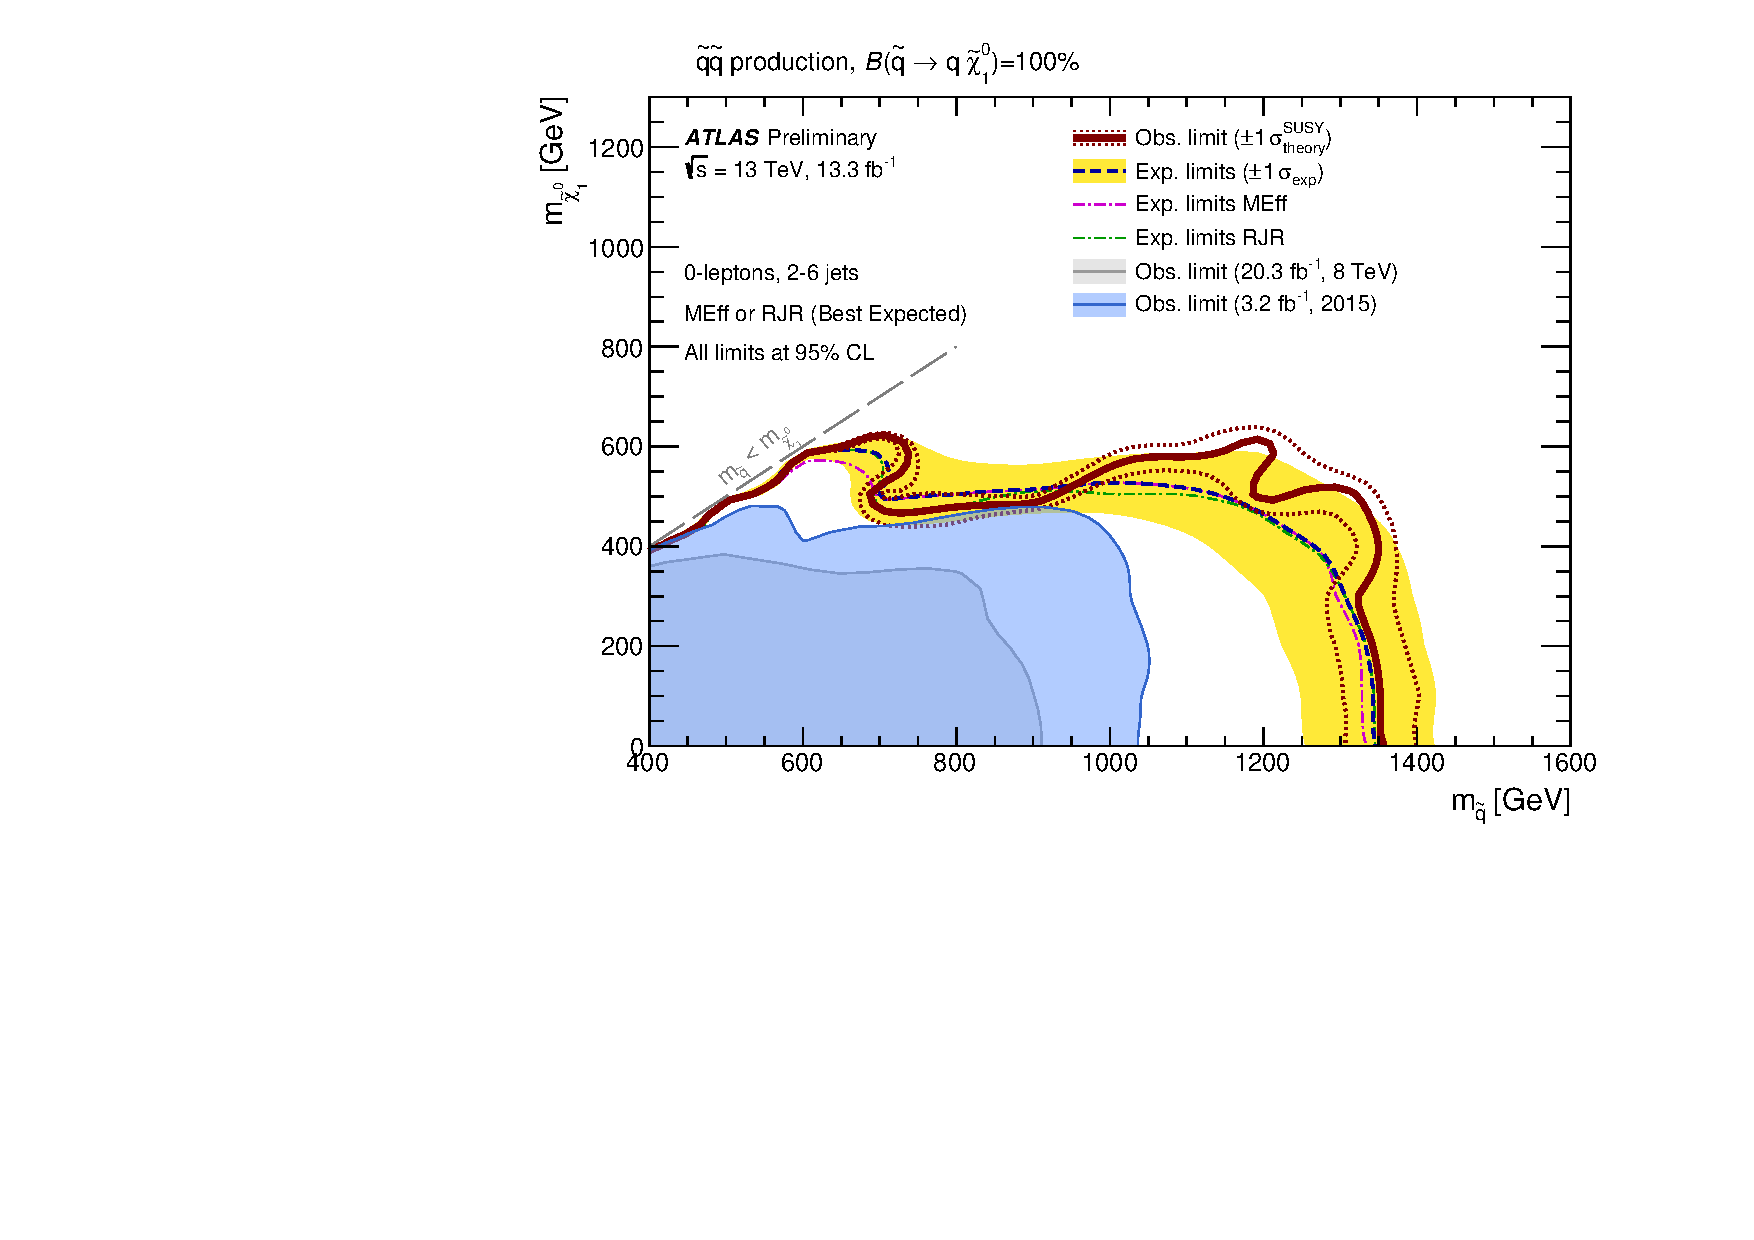
\includegraphics[width=0.49\textwidth]{Figures/fig_09a.pdf}}
\subfigure{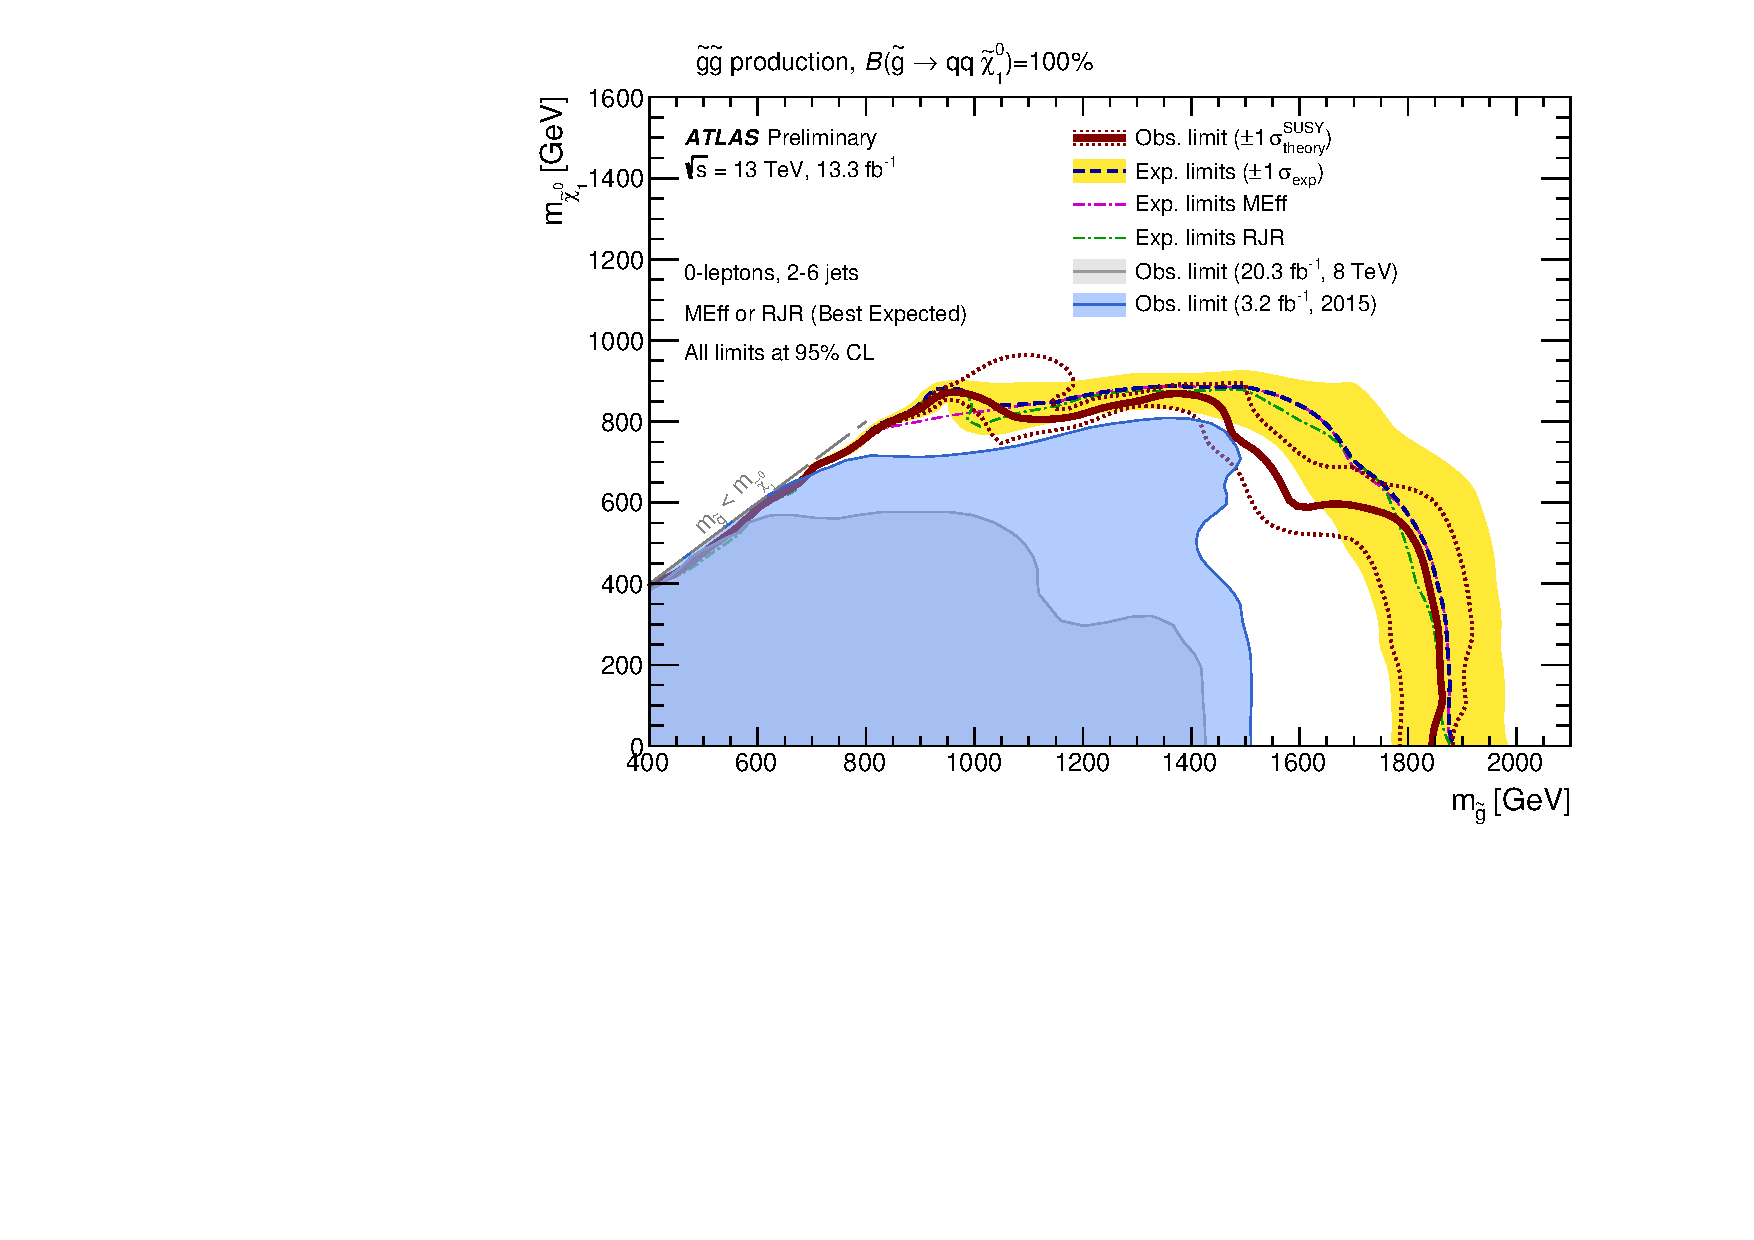
\includegraphics[width=0.49\textwidth]{Figures/fig_09b.pdf}}
\caption{\label{fig:ICHEPLimits} text
}
\end{figure}




The first application of the RJR method was applied to the all hadronic final states. However it would be interesting to explore this view for this final state in more detail, and extend this technique to other topologies, to understand what unique regions of phase space can be probed with the event view.



 that search for signals
where SUSY particles are strongly produced, as well as actively
participates in the search for SUSY in all hadronic states.


In terms of Simplified Models, whereby sparticles are produced and decayed by forced routes, this generally means higher limits on masses of those initially produced sparticle pairs. Regions of Simplified Model phase space that have not been ruled out and are more difficult to observe by traditional search strategies are those for which the mass splitting between the heavier produced sparticle and lightest SUSY particle (LSP) is small, leading to soft visible objects in the final state and low values of reconstructed missing transverse momentum (compressed SUSY spectra). Other challenging scenarios are when new sparticle masses sit on or near masses of known Standard Model particles.


The recent discovery of the Higgs-like boson at 
ATLAS makes the fine-tuning problem real - and argues for renewed focus 
in the search for SUSY.

Early SUSY searches at the LHC primarily focused on scenarios where
large signals were expected, mainly strongly produced light squarks
and gluinos. With no observed signal, these searches now provide the
most stringent limits on SUSY particle masses. As more data was
collected, the SUSY search strategy evolved to target third
generation-mediated gluino production, third generation squark
production (motivated by naturalness arguments), Electroweak
production (ie charginos, neutralinos, and sleptons), and compressed
spectra. With significant boost in LHC's energy and expectation of 100
times more data over the next fifteen years, LHC has a good chance of
finding SUSY if it is accessible.



As sub-convener of the ATLAS SUSY inclusive squark and gluino group,
Louise Heelan, oversees all SUSY analyses that search for signals
where SUSY particles are strongly produced, as well as actively
participates in the search for SUSY in all hadronic states.  The ATLAS
SUSY inclusive squark and gluino group is composed of approximately
140 members, which is itself split into eight paper streams based on
the number of jets and lepton flavors in the final state.
%Searches are generally interpreted in terms of Simplified Models~\cite{Alwall:2008ve,Alwall:2008ag,Alves:2011wf} and various phenomenological models. 
Based on the LHC Run 2 data several papers and conference notes have been made public under the supervision of Heelan~\cite{Aad:2016jxj,Aaboud:2016zdn,Aad:2016qqk,ATLAS-CONF-2015-082,Aad:2016tuk,Aad:2016eki,Aaboud:2016zpr,ATLASCollaboration:2016wlb,ATLAS-CONF-2016-078,ATLAS-CONF-2016-054,ATLAS-CONF-2016-037,ATLAS-CONF-2016-052,ATLAS-CONF-2016-066,ATLAS-CONF-2016-095}. 
To date, there has been no significant evidence of SUSY seen by ATLAS or any other experiment.
Physicists continue their search by exploiting the increasing luminosity at the LHC, and by developing new techniques to search in regions of phase space that are yet ruled out. 
The challenge is finding those holes and finding methods to separate the signal from Standard Model backgrounds.
